\documentclass[CS4402-Notes.tex]{subfiles}
\begin{document}

\section{Modelling}

\subsection{Abstract constraint models}
Constraint modelling is often considered the step to map a well-defined problem statement in a constraint language into a solver-independent constraint model for a constraint solver to solve and find solutions to. Solvers like Savile Row can take a solver-independent model and convert it into its own solver-specific model. However, when viewing constraint models \textit{abstractly}, it can be seen that many combinatorial problems that we wish to tackle exhibit some \textit{common features}.
\n
Many problems require the programmer to find objects such as:
\begin{itemize}
\item (Multi-)sets
\item Relations
\item Functions
\end{itemize}
The abstract constraint model can be written in terms of there patterns. However, the patterns are typically not supported directly by constraint solvers (unlike intensional constraints. As such, the pattens need to be modelled as constrained collections of more primitive objects.
\begin{figure}[H]
\centering
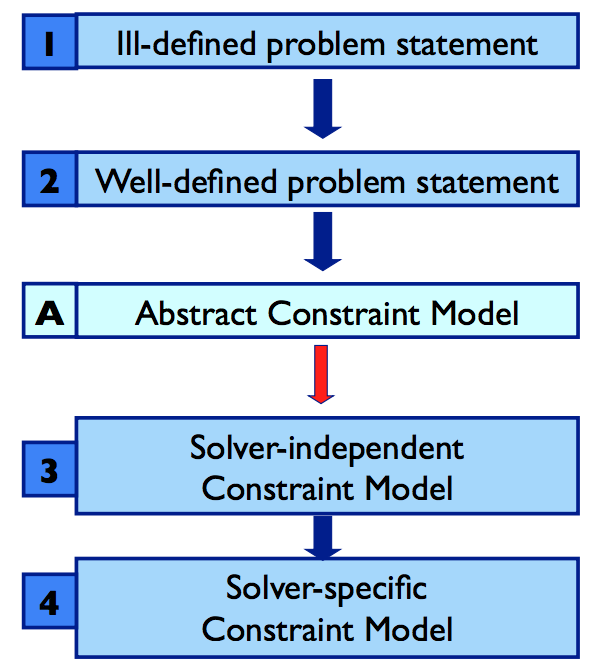
\includegraphics[width=0.5\textwidth, keepaspectratio]{imgs/modelling-steps.png}
\caption{Steps to model a problem for a particular constraint solver.}
\end{figure}
\noindent
This way, the corresponding \textbf{modelling patterns} for representing and constraining these combinatorial objects can be developed and effort is reduced when modelling new problems. Writing abstract constraint models gives a much richer set of types of decision variables, such as sequences, sets and functions and allows the programmer to extract the common features and patterns among different problems. Constraints for these variables and the objective function can also use operators on these new types of objects, such as set union, set relation etc. Finally, the patterns can be combined to model more compex problems.

\subsection{Sequences}
A sequence is defined as an \textbf{ordered list of elements}. It simply has elements in order and repetition is allowed. In the simple case, a sequence in of \textbf{fixed length}, or is \textbf{bounded} by a maximum length. The trickiest case for sequences is when the length is \textbf{unbounded}. Unbounded sequences are a problem because solvers need to use a finite-domain to model the CSP. In these cases, the programmer must be smart to find a bound by reading the problem carefully.
\begin{itemize}
\item 0, 1, 1, 2, 3, 5, 8, 14
\item Turn right, drive 1 mile, turn right, drive 0.5 miles, turn left
\end{itemize}
are examples of sequences. This pattern typically occurs in planning problems, where a sequence of actions is the solution to transform the initial state of the problem into a goal state. Other examples include Langford's problem and the Bombastic problem.

\subsubsection{Fixed-length sequences}
Fixed-length sequences are problems of the form:
\begin{itemize}
\item Given \textbf{n}
\item Find a sequence of objects of length \textbf{n}
\item Such that ...
\end{itemize}
For example the magic sequence problem (CSPLib 19):
\begin{itemize}
\item Given \textbf{n}
\item Find a sequence \textbf{S} of integers $s_{0}, ..., s_{n}$
\item Such that there are $s_{i}$ occurrences of $i$ in \textbf{S} for each $i$ in $0, ..., n$.
\end{itemize}
For the problem instance $n = 9$, a possible solution would be $6, 2, 1, 0, 0, 0, 1 , 0, 0, 0$
\n
To model fixed-length sequences, the most straightforward model is to use an array of decision variables indexied $1...n$ where the domains are the objects to be found.
\begin{figure}[H]
\centering
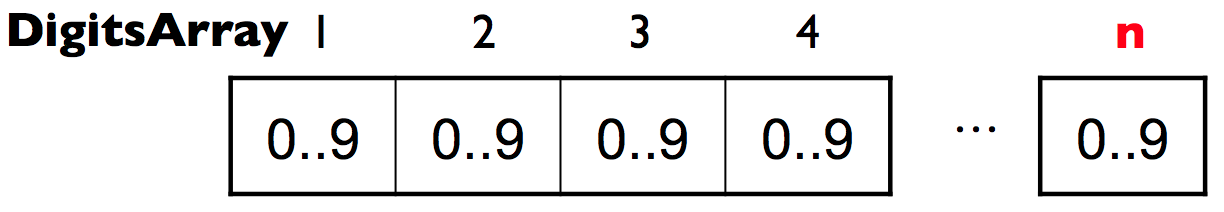
\includegraphics[width=0.8\textwidth, keepaspectratio]{imgs/digits-array.png}
\caption{Array of decision variables 1 to n with their domain specified in an array.}
\end{figure}
\noindent
As a constraint, this can be written as follows:
\begin{lstlisting}
  Forall i in 0..n .
      No. of occurences of i in S of i is S[i]
\end{lstlisting}
Depending on the constraint language being used, this statement may need to be expressed more or less concisely. For example, Essence Prime has a constraint \texttt{gcc(X, Vals, C)} which states that for each non-decision expression \texttt{Vals[i]}, the number of occurrences of \texttt{Vals[i]} in \texttt{X} equals \texttt{C[i]}.
\begin{lstlisting}[caption={The Magic Sequence problem modelled in Essence Prime.}]
  language ESSENCE' 1.0

  given n : int
  find x: matrix indexed by [int(0..n)] of int(0..n)

  such that
  gcc(x, [i | i : int(0..n)], x)
\end{lstlisting}
\begin{itemize}
\item \texttt{x} is the array whose values we are counting and is represented by a matrix of decision variables
\item \texttt{[i | i : int(0..n)]} is the list of values to count, which is a matrix of non-decision variables. The syntax here is a comprehension to produce the values \texttt{[0,1...,n]}
\item \texttt{x} is used a second time here as the number of occurrences of each value, as it is the same as the value that is being counted
\end{itemize}

\subsubsection{Bounded-length sequences}
Bounded-length sequences are similar to fixed-length sequences, except that the length cannot exceed the maximum. The problems come in the form:
\begin{itemize}
\item Given \textbf{n}
\item Find a sequence of objects of length \textbf{at most n}
\item Such that ...
\end{itemize}
The Kiselman Semigroup Problem (KSP) is an example of a problem with infinite domain, but can be bound to a maximum length depending on the problem instance. The problem states that:
\begin{itemize}
\item Given $n$, a positive integer
\item Find a sequence of integers drawn from $1..n$
\item Such that between every pair of occurrences of an integer $i$, there exists an integer greater than $i$ and an integer less than $i$
\end{itemize}
An example solution for $n = 3$ would be $2, 3, 1, 2$. In the definition of this problem, it can be seen that it is not finite. To \textit{Find a sequence of integers drawn from $1..n$}, the sequence can be infinitely long. This is a problem because we want to map the abstract constraint model down to a finite-domain CSP and this is not possible with an infinite domain in the abstract model. To deal with this, we must derive a finite domain for KSP. Notice that there can be at most 1 occurences of 1 and $n$. Likewise:
\begin{itemize}
\item At most 2 occurences of 2 and $n - 1$
\item At most 4 occurences of 3 and $n - 2$
\end{itemize}
From this pattern, we can derive a maximum sequence length of $\sum^{n}2^{n/2} - 1$ pairs, which gives a finite domain for the sequence variable. Finally, because we have set a maximum length to the sequence, we may have to use \textbf{dummy variables} in solutions that are less than the maximum length, but still valid solutions.
\n
We have to be careful when using dummy variables, especially if the value of the dummy exists in the domain of the variables as this will create \textbf{equivalence classes} of assignments. In that case it is impossible to tell if the value assigned to the variable is a real value or a dummy value. The solution to deal with this is to choose a \textbf{canonical element} from each class. For example, saying all 0s must appear at the end of the sequence if the dummy value is 0. Then the constraint will make sure to reject all other equivalences. Introducing equivalances during modelling is something that happens very often and one must be aware of this happening to use appropriate measures to counter it.

\subsubsection{Unbounded sequences}
For some problems, the issue of infinite domains cannot be dealt with in a smart way. This usually happens when a bound cannot be derived, or the derived bound is too weak to be useful. Problems with infinite domains are common when modelling planning problems, for example how many steps are needed to evacuate the building? Or how many actions it neeeded to reach the goal state?
\n
Though inefficient, the solution to this is to solve a series of CSPs by incrementally increasing the length of the sequence. Moreover, this method allows the solver to find a solution with the shortest possible sequence.

\subsubsection{Permutations}
Some problems involve finding a sequence of elements where:
\begin{itemize}
\item The elements in the sequence are known
\item The arrangement of elements is not known
\end{itemize}
The goal is then to find a \textbf{permutation} of the sequence that satisfies the constraints. The Travelling Salesman Problem (TSP) is an example of finding permutations, as the network between the cities and distances are all known.

\subsubsection{Viewpoints}
A \textbf{Viewpoint} is a choice of variables and domains sufficient to characterise the problem. In other words, if there is an assignment to the chosen variables, it can be read off a solution to the problem. Note this doesn't say anything about constraints.
\n
For example, when looking for permutations, we can explore two different viewpoints:
\begin{enumerate}
\item Assume that the elements of the permutation are distinct. This leads to a fixed-length viewpoint.
  \begin{figure}[H]
  \centering
  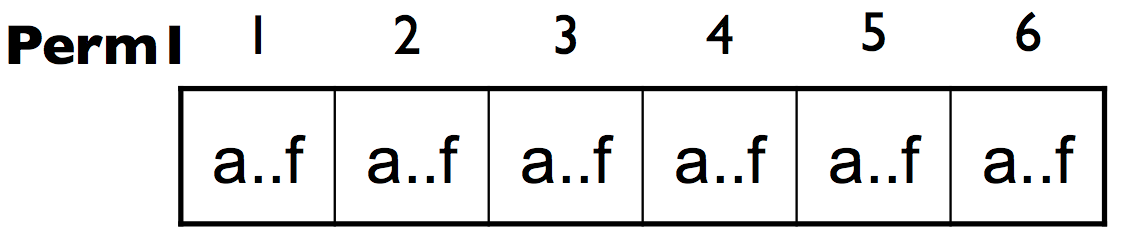
\includegraphics[width=0.6\textwidth, keepaspectratio]{imgs/perm1.png}
  \caption{First viewpoint for a permutation which contains elements $a, ..., f$}
  \end{figure}
\item Alternatively, we know the elements appear in the sequence, so we can index by those elements. The domain values now represent the position in the sequence an element is in.
  \begin{figure}[H]
  \centering
  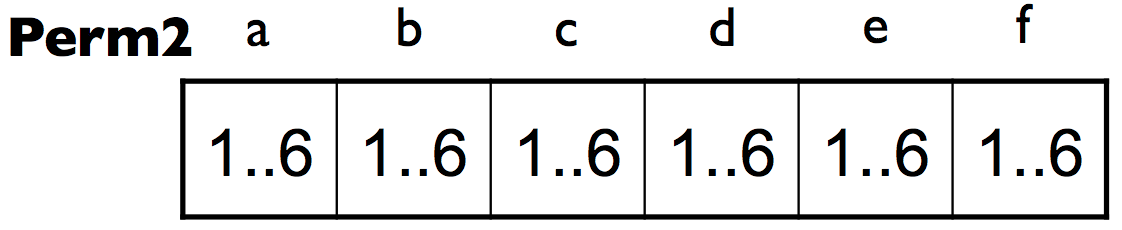
\includegraphics[width=0.6\textwidth, keepaspectratio]{imgs/perm2.png}
  \caption{Second viewpoint for a permutation, using indices instead of elements.}
  \end{figure}
\end{enumerate}
Now there are two different viewpoints to choose from and this will depend on the kind of constraints needed to find a solution. For example, if the constraint is \textit{a and b must be adjacent}, then the second viewpoint it much easier to model with the constraint \texttt{| Perm2[a] - Perm2[b] | = 1}. On the other hand, if the constraint is \textit{The first three letters of the sequence must form an English word}, then it is easier to model the constraitn using the first viewpoint.

\subsection{Sets}
A set is a collection of \textit{distinct} objects not arranged in any particular order. The items in a set must be unique (no duplicates). Examples of set would be $\{1, 2, 3\}$ or \{red, green, blue\}.

\subsubsection{Fixed-cardinality sets}
Consider the following simple problem class:
\begin{itemize}
\item Given $n$ and $s$
\item Find a set of $n$ digits that sum to $s$
\end{itemize}
There are two ways to represent this problem, the \textbf{explicit representation} and \textbf{occurence representation}.

\subsubsection{Explicit representation}
For the explicit representation, an array $E$ is introduces to hold the decision variables indexed by $1..n$, each with a domain of $0..9$. The constraint for the problem is then simply:
\begin{lstlisting}
  AllDifferent(E)
  Sum(E) = s
\end{lstlisting}
However, the issue of equivalence classes once again comes up here. The two sets \{1,3,5,7\} and \{7,3,5,1\} are equivalent as the order does not matter in a set, so a way to deal with this equivalence must be introduced.
\begin{table}[H]
\centering
\begin{tabular}{| c | c | c | c |}
\hline
\textbf{1} & \textbf{2} & \textbf{3} & \textbf{4} \\
\hline
1 & 3 & 5 & 7 \\
\hline
\end{tabular}
\caption{Explicit array representation of the set \{1,3,5,7\}}
\vspace{1cm}
\begin{tabular}{| c | c | c | c |}
\hline
\textbf{1} & \textbf{2} & \textbf{3} & \textbf{4} \\
\hline
7 & 3 & 5 & 1 \\
\hline
\end{tabular}
\caption{Equivalent array reprensentation of the set \{7,3,5,1\}}
\end{table}
A simple way to doing this would be to use ascending order as the canonial element from each class. Then the \texttt{AllDifferent(E)} constraint will be replaced by \texttt{E[1] < E[2] < E[3] < E[4]}.

\subsubsection{Occurrence representation}
Another way to represent sets is with an occurrence representation. This never introduces equivalence classes. It works like an array of binary switches. Following the above example, an occurrence representation $O$ would be an array of 0/1 decision variables indexed by $0..9$:
\begin{table}[H]
\centering
\begin{tabular}{| c | c | c | c | c | c | c | c | c | c |}
\hline
\textbf{0} & \textbf{1} & \textbf{2} & \textbf{3} & \textbf{4} & \textbf{5} & \textbf{6} & \textbf{7} & \textbf{8} & \textbf{9} \\
\hline
0,1 &  0,1 & 0,1 & 0,1 & 0,1 & 0,1 & 0,1 & 0,1 & 0,1 & 0,1 \\
\hline
\end{tabular}
\end{table}
Now we simply need the two constraints:
\begin{lstlisting}
  sum(O) = n
  O[1] + 2O[2] + 3O[3] + ... + 9O[9] = s
\end{lstlisting}
The first constraint only allows $n$ 1s to be filled in the occurrence array and the second constraint is the constraint for the sum of digits.
\n
Both explicit representation and occurrence representation have their advantages and disadvantages. For some problems, an explicit representation may introduce equivalence classes and be more complicated to specify a constraint. For example, if we wanted to say \textit{if 5 is in the set, then so is 4}, this would need a constraint that takes more computation in the explicit representation.
\begin{figure}[H]
\begin{minipage}{0.42\textwidth}
\begin{lstlisting}[caption={Explicit representation}]
Forall j in 1..n .
    If (E[j] = 5)
        Exists i in 1..j-1 . E[i] = 4
\end{lstlisting}
\end{minipage}
\hspace*{\fill}
\begin{minipage}{0.42\textwidth}
\begin{lstlisting}[caption={Occurrence representation}]
(O[5] = 1) -> (O[4] = 1)
\end{lstlisting}
\end{minipage}
\end{figure}
\noindent
It should be noted that a combination of explicit and occurrence representations can be used to model problems, for example the intersection of two occurrence representations is an explicit representation. In other words, the two are not mutually exclusive. Obviously, constraints on the original sets have to be modelled appropriately.

\subsubsection{Set constraints}
As sets appear frequently in constraint problems, it is useful to look at how common constraints such as intersection, union and subset are modelled. Any complex constraint can be decomposed to a simple constraint, each of which has at most one operator and possible one equality sign. For example, the complex constraint
\begin{equation}
(A \cup B) \subseteq (C \cap D)
\end{equation}
can be decomposed into three constraints
\begin{align}
  X &= A \cup B \\
  Y &= C \cap D \\
  X &\subseteq Y
\end{align}

\subsubsection{Set intersection}
The set intersection constraint can be modelled with both the explicit and occurrence representations. Take the simple constraint $A \cap B = C$ where $A$ and $B$ are sets of digits (domain 0..9), an occurrence representation would model it as the following three arrays
\begin{figure}[H]
\centering
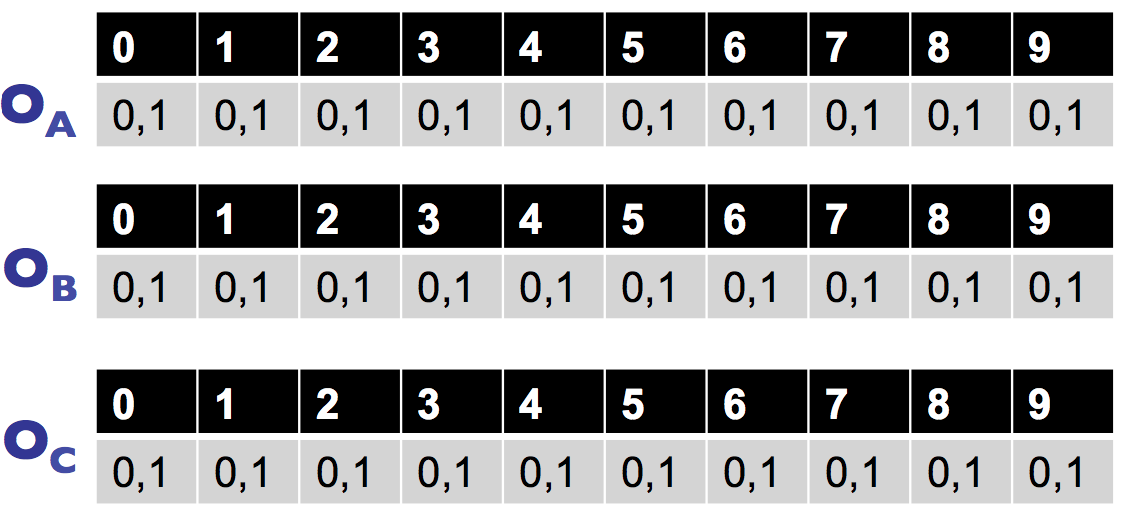
\includegraphics[width=0.7\textwidth, keepaspectratio]{imgs/intersection-occurrence.png}
\caption{Three arrays of switches that map to $A, B$ and $C$.}
\end{figure}
\noindent
with the constraint
\begin{lstlisting}
  Forall i in 0..9 .
    O$_{\texttt{C}}$[i] = O$_{\texttt{A}}$[i] $\times$ O$_{\texttt{B}}$[i] 
\end{lstlisting}
To use explicit representation here would be more complicated and require more complex constraints.
\begin{figure}[H]
\centering
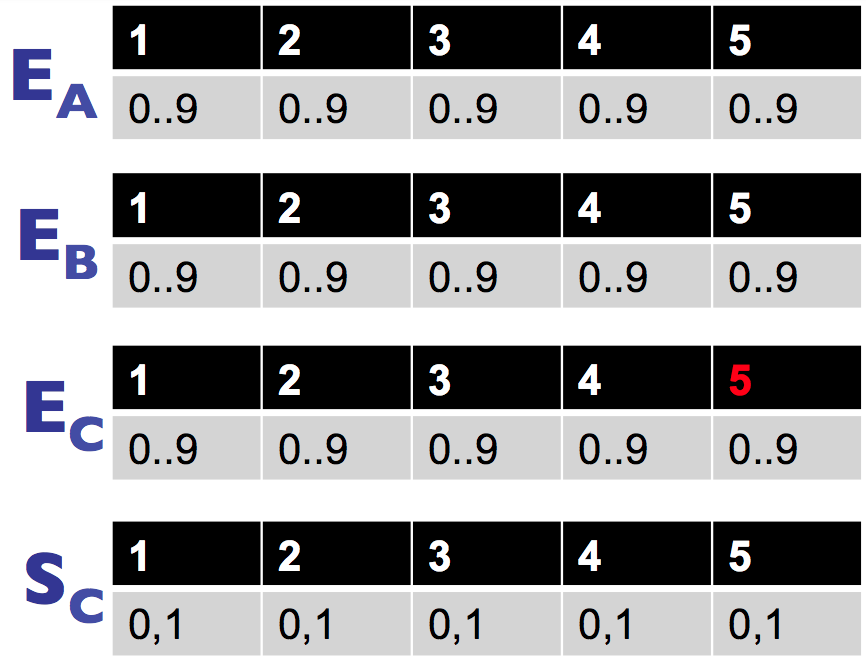
\includegraphics[width=0.6\textwidth, keepaspectratio]{imgs/intersect-explicit.png}
\caption{Arrays for explicit representation of set intersection. Cardinality of 5.}
\end{figure}
\noindent
Each array represents the 5 values in the sets $A, B, C$, but the constraint to expresss the intersection is more complicated. Furthermore, it requires an extra marker array \texttt{S$_{\texttt{C}}$}.
\begin{lstlisting}
  Forall d in 0..9 .
    Forall i in 1..5 .
      If (E$_{\texttt{A}}$[i] = E$_{\texttt{B}}$[i]) && (E$_{\texttt{B}}$[i] = d) . 
        d must appear in E$_{\texttt{C}}$[i]
\end{lstlisting}

\subsubsection{Set union}
The same arrays as in set intersection can be used to model the set union $A \cup B  = C$ simply with a different constraint for an occurrence representation.
\begin{lstlisting}
Forall i in 0..9 . 
  O$_{\texttt{C}}$[i] = (O$_{\texttt{A}}$[i] = 1 $\vee$ O$_{\texttt{B}}$[i] = 1)
\end{lstlisting}
Again this will be more complicated using an explicit representation which will be omitted here.

\subsubsection{Set subset}

\subsection{Multisets}
A multiset (sometimes referred to as ``bags'') is like a set except that duplicate values \textit{are} allowed. They are also not arranged in any particular order and are typically characterised by the number of times each obejct occurs in the multiset. The multiset pattern occurs in places like the packing problem, for example a bag with a number of coloured balls.
\n
Like sets, we must bound the domain of a multiset to be finite. For example,
\begin{itemize}
\item Let $S$ be a finite set of size $n$.
\item The domain ``set of $S$'' comprises of every set whose elements are members of $S$. This domain is the \textbf{power set} of $S$ with size $2^{n}$.
\item The domain ``multiset of $S$'' will comprise of every finite multiset whose elements are all members of $S$. This will have an infinite domain as long as $S$ is non-empty due to infinite repetition.
\end{itemize}
To ensure that the multiset of $S$ is finite, we must bound either the total number of elements in the multiset, or bound the number of occurrences of each value.

\subsubsection{Explicit representation}


\subsubsection{Occurrence representation}
In the occurrence representation of multisets, instead of using 0 or 1 as values in the array, the array is extended to allow multiple occurrences.

\subsection{Relations}
Relations are an assignment of truth values to tuples of values. For example, in the set $P = \{\text{Bill}, \text{Bert}, \text{Tom}\}$, a binary relation \textit{like} can be defined between two people from the set $P$. We might assign the tuple $<$Bill, Bert$>$ and $<$Bert, Tom$>$ to be true and false for all other combinations.
\end{document}
